\documentclass[runningheads,a4paper]{llncs}

\usepackage[usenames, dvipsnames]{color}
\usepackage{times}
\usepackage{xspace}
\usepackage{textcomp}
\usepackage{wrapfig}
\usepackage{url}
\usepackage{amsmath, amssymb}
\usepackage{graphicx}
\usepackage[protrusion=true,expansion=true]{microtype}

\usepackage{alltt}
\usepackage{appendix}
\newcommand{\keywords}[1]{\par\addvspace\baselineskip
\noindent\keywordname\enspace\ignorespaces#1}

\pdfinfo{/Title (Dedalus: Datalog in Time and Space)}

\usepackage{txfonts}
\newcommand{\Tau}{\mathcal{T}}
\newcommand{\SDedalus}{\mathcal{S}}
\newcommand{\Consts}{\mathcal{C}}
\newcommand{\Vars}{\mathcal{A}}
\newcommand{\pos}{\_pos}
\newcommand{\nega}{\_neg}

\newcommand{\jmh}[1]{{\textcolor{red}{#1 -- jmh}}}
\newcommand{\paa}[1]{{\textcolor{blue}{#1 -- paa}}}
\newcommand{\rcs}[1]{{\textcolor{green}{#1 -- rcs}}}
\newcommand{\nrc}[1]{{\textcolor{magenta}{#1 -- nrc}}}
\newcommand{\wrm}[1]{{\color{BurntOrange}{#1 -- wrm}}}
\newcommand{\smallurl}[1]{{\small \url{#1}}}

\def\lang{\textsc{Dedalus}\xspace}
\def\slang{\textsc{Dedalus\ensuremath{_{{0}}}}\xspace}
\newcommand{\naive}      {na\"{\i}ve\xspace}
\newcommand{\Naive}      {Na\"{\i}ve\xspace}

\newenvironment{Dedalus}{
\vspace{0.5em}\begin{minipage}{0.95\textwidth}%\linespread{1.3}
\begin{alltt}\fontsize{9pt}{9pt}\selectfont}
{\end{alltt}\end{minipage}\vspace{0.5em}}

\newcommand{\dedalus}[1]{\texttt{\fontsize{9pt}{9pt}\selectfont #1}}


\begin{document}

\mainmatter  % start of an individual contribution

\title{{\Large{\bf\lang}}:
Datalog in Time and Space} 

\titlerunning{{\bf\lang}: Datalog in Time and Space}

\author{Peter Alvaro\inst{1} \and William R. Marczak\inst{1} \and Neil Conway\inst{1} \and \\ Joseph M. Hellerstein\inst{1} \and David Maier\inst{2} \and Russell Sears\inst{3}}

\authorrunning{Alvaro et al.}

\institute{University of California, Berkeley:
\email{\{palvaro, wrm, nrc, hellerstein\}@cs.berkeley.edu}
\and
Portland State University:
\email{maier@cs.pdx.edu}
\and
Yahoo! Research:
\email{sears@yahoo-inc.com}
}



\maketitle

\begin{abstract} 
Recent research has explored using Datalog-based
languages to express a distributed system as a set of logical
invariants.  Two properties of distributed
systems proved difficult to model in Datalog.  First, the state of any such system
evolves with its execution.  Second, deductions in these systems may be
arbitrarily delayed, dropped, or reordered by the unreliable network links
they must traverse.  Previous efforts addressed the former by extending
Datalog to include updates, key constraints, persistence and events, and
the latter by assuming ordered and reliable delivery while ignoring delay.
These details have a semantics outside Datalog, which increases the complexity of
the language and its interpretation, and forces programmers to
think operationally.  We argue that the missing component from these previous
languages is a notion of {\em time}.

In this paper we present {\bf \lang}, a
foundation language for programming and reasoning about distributed systems.
\lang reduces to a subset of Datalog with negation, aggregate
functions, successor and choice, and adds an explicit notion of logical time
to the language.
We show that \lang provides a declarative foundation for the two signature features of 
distributed systems: mutable state, and asynchronous processing and communication.
Given these two features, we address two important properties of programs in 
a domain-specific manner: a notion of {\em safety} appropriate to non-terminating computations, 
and {\em stratified} monotonic reasoning with negation over time.  We also provide conservative syntactic checks
for our temporal notions of safety and stratification.  Our experience implementing 
full-featured systems in variants of Datalog suggests that \lang is well-suited to the specification of
rich distributed services and protocols, and provides both cleaner semantics and richer tests of correctness.

\keywords{Datalog, distributed systems, logic programming, temporal logic}
\end{abstract}

\section{Introduction}
%Our research is motivated by two hard problems in distributed systems.  First,
\wrm{show examples of the problems (not necessarily code) -- evolving state and unreliable communication}

%Distributing any system introduces nondeterminism.  For example, one may
%distribute a computation over many inexpensive, but unreliable, commodity
%machines (e.g. RAID).  The status of internet links and widely distributed
%nodes is inherently more unreliable than multiple cores on a single die, or
%multiple CPUs in a single computer.  

%We present {\bf \lang}, a foundation language for programming and
%reasoning about distributed systems.  

%We correct deficiencies in earlier attempts, and introduce a compelling notion
%of non-determinism in the language.  We specifically use non-determinism to
%reason about {\em when} a deduction becomes visible, including the possibility
%that the deduction will never be visible.  Programmers can constrain this
%non-determinism by using well-studied techniques in distributed systems, such as
%Lamport Clocks 


Traditional database systems are based on declarative query languages that
specify transformations as dataflows over an updatable store.  Such query
languages are either not expressive enough to capture common programming
constructs \wrm{like what?}, or are at best awkward to use in this fashion.
\wrm{todo: transition that explains Datalog's birth from these languages... I
don't know enough to write it} The family of logic-based database languages, of
which Datalog is the progenitor, represent expressive programming languages
that produce similar dataflow representations.  Datalog is purely deductive: a
program specifies the rules by which the derived relations are populated based
on a static database, which is never updated.  Recent programming language
research has explored the use of Datalog-based languages for expressing
distributed systems.  Because the state of any complex system evolves with its
execution, these efforts were forced to extend the Datalog model by admitting
updates, additions and deletions of the EDB.  Unfortunately, these previous
attempts were plagued with ambiguities about how and when state changes occur
and become visible, putting a heavy burden on the programmer to ensure even
simple properties, such as atomicity of updates over time.

In contrast to reasoning about state change procdurally, \lang observes
that this concept is intuitively expressed as invariants over {\em time}.  In
this work, we present a formal model of Datalog augmented with time extensions.
By reifying time as data an introducing it into the logic, \lang eliminates
previous ambiguities, ensures atomicity of updates and makes it possible to
express system invariants that can guarantee liveness properties, a key
challenge in building distributed systems.

\section{\large \bf \lang}
\label{sec:foundation}

\subsection{Preliminary Definitions}

We assume an infinite universe $\mathcal{U}$.

A {\em relation schema} is a pair consisting of a relation name and its arity.  A {\em schema} $\mathcal{S}$ is a set of relation schemas.  As in \wrm{cite Immerman}, we assume the existence of an order.  Thus, all schemas contain the following relational schemas: \dedalus{lt} -- a relation of arity two that is true whenever the second argument is greater than the first (we will write this relation in infix form using the \dedalus{<} symbol) -- \dedalus{suc} -- a relation of arity two that defines a total order over $\mathcal{U}$ \wrm{different from succ}.

A {\em rule} over a schema $\mathcal{S}$ is a clause of the form:

\begin{Dedalus}
p(\(\bar{X_0}\)) <- b_1(\(\bar{X_1}\)), \ldots, b_n(\(\bar{X_n}\)), !c_1(\(\bar{Y_1}\)), \ldots, !c_m(\(\bar{Y_m}\)).
\end{Dedalus}

where \dedalus{h}, \dedalus{\(b_1\), \ldots, \(b_n\)}, \dedalus{\(c_1\), \ldots, \(c_m\)} are relations in $\mathcal{S}$, and $\bar{X_i}$ and $\bar{Y_i}$ denote a tuple (of the appropriate arity) consisting of variable symbols, constants from $\mathcal{U}$.  Note that we maintain the usual safety restrictions of Datalog rules: any variable symbol $V$ that appears in $\bar{Y_i}$ for some $1 \leq i \leq m$ must also appear in $\bar{X_j}$ for some $1 \leq j \leq n$, but only if $V$ appears in $\bar{X_0}$ or $V$ appears in $\bar{Y_k}$ for some $k \neq i$ -- i.e., variable symbols that only appear in a single negated atom and do not appear in the head need not also appear in a positive atom \wrm{cite ullman}.

\wrm{describe recursion, rule out recursion through negation, define EDB}

A {\em fact} over a relation schema of arity $n$ is a pair consisting of the relation name and an $n$-tuple $(c_1,\ldots,c_n)$, where each $c_i \in \mathcal{U}$.  An instance $\mathcal{I}$ over a schema $\mathcal{S}$ is a set of facts.

Given a schema $\mathcal{S}$, we use $\mathcal{S}^*$ to denote the extension of $\mathcal{S}$ obtained by adding two columns to each relation schema in $\mathcal{S}$, and adding three additional relation schemas to $\mathcal{S}$.  The first additional column, the {\em location specifier}, indicates the ``location'' of the tuple, and the second additional column, the {\em timestamp}, is a natural number representing a logical time.  \wrm{As in...} We call $\mathcal{S}^*$ a {\em spatio-temporal} schema.  The three relations we add are: \dedalus{time}, a unary relation equivalent to $\mathbb{N}$, \dedalus{succ}, a binary relation representing the natural successor relation over $\mathbb{N}$, and \dedalus{node}, a unary relation that represents all locations (the meaning of ``location'' will become clear later).

A {\em spatio-temporal} fact over a relation schema of arity $n$ is a pair consisting of the relation name and an $n+2$ tuple $(l,t,c_1,\ldots,c_n)$ where each $c_i \in \mathcal{U}$, $l \in \dedalus{node}$, and $t = 0$ (all spatio-temporal facts must be supplied with timestamp 0).

A {\em spatio-temporal rule} over a spatio-temporal schema $\mathcal{S}^*$ is a rule of one of the following three forms:

A {\em deductive} rule:
\begin{Dedalus}
p(L,T,\(\bar{X_0}\)) <- b_1(L,T,\(\bar{X_1}\)), \ldots, b_n(L,T,\(\bar{X_n}\)), !c_1(L,T,\(\bar{Y_1}\)), \ldots, !c_m(L,T,\(\bar{Y_m}\)).
\end{Dedalus}

An {\em inductive} rule:
\begin{Dedalus}
p(L,S,\(\bar{X_0}\)) <- b_1(L,T,\(\bar{X_1}\)), \ldots, b_n(L,T,\(\bar{X_n}\)), !c_1(L,T,\(\bar{Y_1}\)), \ldots, !c_m(L,T,\(\bar{Y_m}\)), succ(T,S).
\end{Dedalus}

An {\em asynchronous local} rule:
\begin{Dedalus}
p(L,S,\(\bar{X_0}\)) <- b_1(L,T,\(\bar{X_1}\)),\ldots,b_n(L,T,\(\bar{X_n}\)), !c_1(L,T,\(\bar{Y_1}\)), \ldots, !c_m(L,T,\(\bar{Y_m}\)), time(S), S > T, choice((L, T, \(\bar{B}\)),(S)).
\end{Dedalus}

An {\em asynchronous communication} rule:
\begin{Dedalus}
p(D,S,\(\bar{X_0}\)) <- b_1(L,T,\(\bar{X_1}\)),\ldots,b_n(L,T,\(\bar{X_n}\)), !c_1(L,T,\(\bar{Y_1}\)), \ldots, !c_m(L,T,\(\bar{Y_m}\)), time(S), S > T, choice((L, T, \(\bar{B}\)),(S)), node(D).
\end{Dedalus}

where all symbols are as defined before, $\bar{B}$ is a list of all of the distinct variable symbols in $\bar{X_1}, \ldots, \bar{X_n}, \bar{Y_1}, \ldots, \bar{Y_m}$; \dedalus{D} and \dedalus{L} are variable symbols that may also appear in $\bar{B}$, \dedalus{T} and \dedalus{S} are variable symbols that may not appear in $\bar{B}$, and \dedalus{choice} is the construct of Sacc\`{a} and Zaniolo~\cite{sacca-zaniolo}, which we will presently describe.

A \lang {\em program} is a set of spatio-temporal rules over some spatio-temporal schema $\mathcal{S}^*$.  Note that a given set of rules over a schema may give rise to many different \lang programs, depending on which type of spatio-temporal rule each rule is converted into, and depending on where or if the variable $D$ appears in the body in asynchronous communication rules.

A \lang {\em instance} is a program with a set of spatio-temporal facts specified for EDB relations.

\noindent
\textbf{Syntactic sugar for space-time in \lang:}
The restrictions on temporal and location attributes suggest a natural syntactic sugar to improve readability.  Given the unification requirements for location and temporal attributes in rule bodies, we can omit these attributes from predicates without risk of ambiguity.  

The three temporal classes of rules listed above can be distinguished by annotating inductive head predicates with \dedalus{@next}, and asynchronous head predicates with \dedalus{@async}; simple deductive rules have no head annotation. 
Communication rules must include the location attribute of their head predicate; by definition this is a different variable than that of the body predicates.
 Given these conventions, the presence of appropriate \dedalus{successor}, \dedalus{choice} and \dedalus{node} predicates in the body are implicit, and can be omitted.  The result is a syntax that reads like a simple temporal variant of Datalog.

Deductive:
\begin{Dedalus}
p(\(\bar{X_0}\)) <- b_1(\(\bar{X_1}\)), \ldots, b_n(\(\bar{X_n}\)), !c_1(\(\bar{Y_1}\)), \ldots, !c_m(\(\bar{Y_m}\)).
\end{Dedalus}

Inductive:
\begin{Dedalus}
p(\(\bar{X_0}\))@next <- b_1(\(\bar{X_1}\)), \ldots, b_n(\(\bar{X_n}\)), !c_1(\(\bar{Y_1}\)), \ldots, !c_m(\(\bar{Y_m}\)).
\end{Dedalus}

Asynchronous local:
\begin{Dedalus}
p(\(\bar{X_0}\))@async <- b_1(\(\bar{X_1}\)), \ldots, b_n(\(\bar{X_n}\)), !c_1(\(\bar{Y_1}\)), \ldots, !c_m(\(\bar{Y_m}\)).
\end{Dedalus}

Asynchronous communication:
\begin{Dedalus}
p(#D,\(\bar{X_0}\))@async <- b_1(#L,\(\bar{X_1}\)), \ldots, b_n(#L,\(\bar{X_n}\)), !c_1(#L,\(\bar{Y_1}\)), \ldots, !c_m(#L,\(\bar{Y_m}\)).
\end{Dedalus}

Asynchronous communication rules require the body location specifier to be explicit, because it may be unified with other body attributes.


%\vspace{1em}
%\noindent 
%\textbf{Predicate Dependence Graphs in \lang}: 
%A \lang program's {\em predicate dependency graph}~\cite{ullmanbook} PDG is 
%a directed graph that has one node per predicate, and an edge from \dedalus{q} to \dedalus{p} if predicate \dedalus{p} appears in the head of a rule with \dedalus{q} in its body.  If \dedalus{q} is negated, or a \dedalus{count} appears in the head of the rule, we mark the edge as negated.  If the rule is inductive or asynchronous, we annotate the edge with the rule type.  The PDG omits the \dedalus{time} and \dedalus{successor} predicates, and the nodes and edges for \dedalus{choice}.  We write $\dedalus{q} \to \dedalus{p}$ if there exists a path following forward edges from \dedalus{q} to \dedalus{p}.  We write $\dedalus{q} \nrightarrow \dedalus{p}$ if there exists a forward path from \dedalus{q} to \dedalus{p} that crosses a negated edge.  We write $\dedalus{q} \circleright \dedalus{p}$ if all forward paths from \dedalus{q} to \dedalus{p} traverse an asynchronous or inductive edge.  We write $\dedalus{q} \Diamondright \dedalus{p}$ if at least one forward path from \dedalus{q} to \dedalus{p} traverses an async edge. 



\subsection{Semantics}
One interpretation of a \lang instance is given by the possible worlds of the stable model semantics~\cite{stable-model}.  We do not review the stable model semantics here -- the only salient detail is the interaction of\dedalus{choice} with the stable model semantics.  \dedalus{choice} induces a separate stable model foreach possible sequence of choices of timestamps.  Note that without \dedalus{choice} -- i.e., without any asynchronous local or asynchronous communication rules -- a \lang program has a unique stable model, because it is locally stratified.

There are two potential problems with considering a stable model as the meaning of a \lang instance.  First, every program with at least one asynchronous rule has infinitely many stable models.  Not all of these stable models may be meaningfully different.  Second, a stable model of a \lang program may itself be infinite.  We address both concerns in our definition of an {\em ultimate model}.

\begin{example}
\label{ex:flipflop}
A \lang program with an infinite stable model.

\begin{Dedalus}
flipflop(Y,X)@next \(\leftarrow\) flipflop(X,Y);
flipflop(1,2)@1;
\end{Dedalus}

\dedalus{flipflop(1,2)} is true at all odd times, and \dedalus{flipflop(2,1)} is true at all even times.  Thus, \dedalus{flipflop(1,2)} and \dedalus{flipflop(2,1)} are each cyclic with period 2.
\end{example}

\wrm{explain the ultimate model in terms of defining an output schema, and everything that is ever asserted into that output schema is part of the output}.



\subsection{Operational Interpretation}
\label{sec:operational}

Our goal in defining an operational formalism is to demonstrate that our model-theoretic view of distributed systems corresponds to the real-world behaviors of such systems.

\wrm{describe what kind of system this models, how it would be executed}
\wrm{describe failure model -- all messages eventually delivered}


\section{Time, State and Order}
\label{sec:stateupdate}

%%\linebreak
\begin{quote}
%
\emph{Time is a device that was invented to keep everything from
happening at once.}\footnote{Graffiti on a wall at Cambridge
University~\cite{scheme}.}
%
\end{quote} 

%Recall that by an event, we mean a \lang fact.
%The transitive consequences
%(via deductive rules) of events are likewise events and hold atomically in the
%same timestep with their premises.  However,

As we showed in the previous section, logical time may be used as a 
``source of monotonicity'' to restore a meaningful, temporal interpretation to otherwise
semantically ambiguous constructs like updateable state and orderly processing.  
Many common motifs in systems programming
(distributed and otherwise) follow a similar pattern of restricted nonmonotonicity, in 
which consequences of deductions are deferred in time.  In this section, we demonstrate
the expressivity of \lang by building a collection of stateful and orderly contructs,
most of which employ the careful use of nonmonotonic reasoning deferred in time.
We also introduce a convenience notation in the form of a simple macro language
for many of these common patterns.

%%\noindent{}In an asynchronous system, the programmer will in general not be able to
%%predict when, or in what order, events arrive from other nodes.  Additionally,
%%some events may need to be handled over time \jmh{vague}, requiring state-oriented motifs
%%such as persistence and mutability.  In this section, we construct a library of
%%\lang constructs to capture these two uses of order.

%Given our definition of \lang, we now address the persistence and mutability
%of data across time: a signature feature of distributed systems---and systems
%in general.
%---for which we provide a model-theoretic foundation.

%The intuition behind \lang's \dedalus{successor} relation is that it models the
%passage of (logical) time.  In our discussion, we will say that facts with
%lower time suffixes occur ``before'' atoms with higher ones.  The constraints
%we imposed on \lang rules restrict how deductions may be made with respect to
%time.  First, rules may only refer to a single time suffix variable in their
%body, and hence {\em cannot join across different ``timesteps''}.  Second,
%rules may specify deductions that occur concurrently with their ground facts,
%\wrm{define ground fact somewhere} in the next timestep, or at some arbitrary
%time, including times before their ground facts.

%This notion of time allows us to consider the contents of the EDB---and hence
%a model of an instance---with respect to an ``instant in time'': we simply
%bind the time suffixes ($\DT$) of all body predicates to a constant.  Because
%this produces a sequence of models (one per timestep), it gives us an intuitive
%and unambiguous way to declaratively express persistence and state changes
%across time.  In this section, we give examples of language constructs
%that capture state-oriented motifs such as persistent relations,
%deletion and update, sequences, and queues.

\subsection{State in Logic}

\jmh{Back this up with formalism: can't do a flip/flop in Datalog (Chandra/Harel, right?).  This discussion does tee up the question of whether something more traditional like Datalog-neg would have been enough for us ... might be sufficient to simply toss in a result about Turing completeness of Dedalus.  I realize your point here is more practically-minded and illustrative, but then maybe this intro is off target for this section.  Still I think an expressivity subsection in the paper would be nice.}


Logic languages naturally model the accumulation of information: deduction in 
the broadest sense tells us, given what we already know, what follows from it.  However, systems
programming frequently requires us to model information that may disappear or change
over time.  In this section we model persistence, both immutable and dynamic, as
\emph{induction} over time, and provide a convenience notation for declaring certain
relations as ``persistent.''


\subsubsection{Simple Persistence}
%
A fact in predicate $p$ at time $\DT$ may provide ground for deductive rules at
time $\DT$, but may only provide ground for deductive rules in timesteps
greater than $\DT$ if it is persisted.  One way to persist all facts in a
predicate $p$ is to use a {\em simple persistence rule}:

\dedalus{p\pos($A_1$,$A_2$,[...],$A_n$)@next $\leftarrow$
p\pos($A_1$,$A_2$,[...],$A_n$);}

\noindent A rule of this form ensures that a $p$ fact true at time $i$ will be
true $\forall j \in \mathbb{N} : j >= i$.


\subsubsection{Mutable State}
\label{sec:mutable}

Simple persistence rules cannot model deletions and updates of a fact, because
they express an unbroken induction over time.  One way to allow the induction
to be broken is to add a \dedalus{p\nega} subgoal to the body of a simple
persistence rule:

\begin{dedalus}
p\_pos($A_1,A_2,[...],A_n$)@next $\leftarrow$
\end{dedalus}

\hspace{5mm}
\begin{dedalus}
p\_pos($A_1,A_2,[...],A_n$),
\end{dedalus}

\hspace{5mm}
$\lnot$
\begin{dedalus}
p\_neg($A_1,A_2,[...],A_n$);
\end{dedalus}

\noindent If, at any time $k$, we have a fact
\dedalus{p\nega($\overline{C}$)@k}, then we do not deduce a
\dedalus{p\pos($\overline{C}$)@k+1} fact.  Furthermore, we do not deduce a
\dedalus{p\pos($\overline{C}$)@j} fact for any $j > k$, unless this
\dedalus{p\pos} fact is re-derived at some timestep $j > k$ by another rule.
This corresponds to the intuition that a persistent fact, once stated, is true
until it is retracted.

%%\newtheorem{example}{Example}
\begin{example}
Consider the following \lang instance:\rcs{introduce p predicate?}

%%p\pos(A, B) \(\leftarrow\) p(A, B);
\begin{Dedalus}
p\pos(A, B)@next \(\leftarrow\) p\pos(A, B), \(\lnot\)p\nega(A, B);

p(1,2)@101;
p(1,3)@102;
p\nega(1,2)@300;
\end{Dedalus}

It is easy to see that the following facts are true: \dedalus{p(1,2)@200},
\dedalus{p(1,3)@200}, \dedalus{p(1,3)@300}.  However, \dedalus{p(1,2)@301} is
false because it was ``deleted'' at timestep \dedalus{300}.
\end{example}

Since mutable persistence occurs frequently in practice, we provide the
\dedalus{persist} template, which takes two arguments: a predicate name and
its arity.  The macro expands to the corresponding mutable persistence rule,
and rewrites the current program in such a way that any references to the given
predicate (say \dedalus{p}) in rule bodies or heads are replaced by references
to its positive relation (e.g., \dedalus{p\_pos}), except for references in the
head of a rule which prefix \dedalus{p} with the distinguished \dedalus{delete}
keyword---these are replaced with \dedalus{p\_neg}.  The above
\dedalus{p\_pos} persistence rule may be equivalently specified as
\dedalus{persist[p,  2]}.

Mutable persistence rules enable {\em updates}.  For some time $\DT$, an update
is any pair of facts:

\begin{dedalus}
p\nega($\overline{C})@\DT;$
\end{dedalus}

\begin{dedalus}
p\pos($\overline{D})@\DT+1$;
\end{dedalus}


\noindent Intuitively, an update represents deleting an old value of a
tuple and inserting a new value.  Every update is {\em atomic across
  timesteps}, meaning that the old value exists during timestep $\DT$
when the new value is derived.  During the evaluation of timestep
$\DT+1$ the new value exists, and the old does not.

\subsubsection{Assignment and Committed Choice}

The assignment primitive provided by most imperative languages is a special case
of update without deletion.  We can model the (destructive) assignment of sets
of values to keys in the following way:

\begin{Dedalus}
log(A, B)@next \(\leftarrow\) condition(A, B);
log(A, B)@next \(\leftarrow\) log(A, B), \(\lnot\)condition(A, _);
\end{Dedalus}

The pair of rules above will cause {\em log} to associate with $A$ the ``most
recent'' set of $B$ values appearing in {\em condition}.  If {\em condition(A,
B)} respects the functional dependency $A \to B$, then \dedalus{log} will
associate only the ``most recent'' $B$ value with each $A$.

The mirror image of assignment is committed choice~\cite{committedchoice},
which associates the first
value(s) of $B$ with $A$.  Committed choice ``seals'' the value of \dedalus{B} such that ``future''
insertions into \dedalus{condition} cannot cause new rows with the same
\dedalus{A} value to be inserted.

\begin{Dedalus}
log(A, B)@next \(\leftarrow\) log(A, B);
log(A, B)@next \(\leftarrow\) condition(A, B), \(\lnot\)log(A, _);
\end{Dedalus}
%%\subsection{``At Most Once'' event relations}

Assignment and committed choice implement ``last write wins'' and 
``first write wins'' semantics, respectively.

\subsubsection{``At Most Once``}
A common requirement for programs with side-effects outside the control
of the system is ensuring that certain events occur ``at most once.''
Consider a requirement for our shopping cart application 
that only a single checkout response should be generated, even if subsequent
inputs cause the totals to be recalculated.  Hence we want to ensure that the
predicate {\em response} ``fires'' only once, regardless of the number of times 
that {\em status} fires.  This feature can be expressed as a 
specialization of the committed choice pattern.   

\begin{Dedalus}
response(Cli, Ses, Item, Amt) \(\leftarrow\)
  amo\_event(Cli, Ses, Item, Amt);

amo\_event(Cli, Ses, Item, Amt) \(\leftarrow\)
  status(Cli, Ses, Item, Amt), 
  \(\lnot\) amo\_log(Cli, Ses, Item, _);

amo\_log(Cli, Ses, Item, Amt)@next \(\leftarrow\) 
  amo\_event(Cli, Ses, Item, Amt);

amo\_log(Cli, Ses, Item, Amt)@next \(\leftarrow\) 
  amo\_log(Cli, Ses, Item, Amt);
\end{Dedalus}

In the subprogram above, the (immutable) predicate {\em amo\_log} serves as a guard
for the predicate {\em amo\_event}, which is true only for the ``first'' assignment
of an $Amt$ value to a grouping of client, session and item identifiers.  Subsequent
occurrences of the {\em status} event for the same group will never fire the second rule.

%But perhaps surprisingly,
%``closing a world'' in this fashion ensures that \dedalus{log} has strictly
%monotonic behavior in all models
%\wrm{commenting out fancy pants diction, so neil doesn't have to}

\paa{introduce 'at most once' as a specialization of committed choice, and
present the macro, which expands to a table (say foo), a log (foo\_log) and an
event (foo\_event) which occurs once if foo occurs at all.}

\subsection{Order in Logic}

\paa{some intro text: pure logic has no notion of order.  distributed systems programming
frequently requires ordering constructs to cope with indeterminacy in message ordering
and to achieve synchronization}

\noindent{}In an asynchronous system, the programmer will in general not be able to
predict when, or in what order, events arrive from other nodes.  When the timing and 
ordering of message arrival affects program results, it may be necessary to instrument
programs with constructs that preserve or restore order at communication boundaries,
or to ensure that simultaneous arrival of messages has the same effect as serial arrival.

\subsubsection{Priority Queues}

\paa{whack this ponderous subsection.  present instead \emph{serializers},
which do what so-called queues below do: enforce 'associativity' by preventing
more that one tuple from being considered per fixpoint.  then present
\emph{ordered queues} (or perhaps the same thing with a better name)
after the discussion of sequences (since OQs use sequences), as a mechanism
for maintaining ordering across async boundaries (familiar from TCP, fifo broadcast,
etc)}

%\paa{shorten this section} While a sequence is a useful construct for
%generating or imposing an ordering on tuples \wrm{seems a bit fishy.  seems
%like it might only be useful for transferring a given order thru async,
%assuming the tuples are already ordered at sender. plus, seqs appears after
%this now}, 

\wrm{i think this might be the wrong way to present queues.  queues don't
necessarily guarantee that ``all things of priority X happen before all things
of priority Y>X''.  the two high order bits of queues are: they prevent things
of different priorities from simultaneously executing, and they enforce kind of
a loose order ``dequeue the lowest priority thing i have thus far''.  ordering
by itself isn't a high-order bit though, because i can sort in one stratum.
it's more this ``online loose order'' which is important.  didn't want to do
too much damage to this section, so i didn't rewrite it yet to conform with
this.}

Some programs will require tuples to be processed in a particular (partial)
data-dependent order, rather than all-at-once, as a set.  For example,
consider a predicate \dedalus{priority\_queue} that represents a series of
tasks.
%to be performed in some predefined order.
Its attributes are two strings---a user and a job---and an integer indicating
the priority of the job in the queue:

\begin{Dedalus}
priority\_queue('bob', 'bash', 200)@123;
priority\_queue('eve', 'ls', 1)@123;
priority\_queue('alice', 'ssh', 204)@123;
priority\_queue('bob', 'ssh', 205)@123;
\end{Dedalus}

A program may desire to serialize the jobs, despite the coincidence of the
\dedalus{priority\_queue} events in logical time.

%Depending on the program that implements the balance update, several behaviors
%are possible.
%Given this schema, we note that a program would likely want to process
%\dedalus{priority\_queue} events individually in a data-dependent order, in
%spite of their coincidence in logical time.  

%%It is difficult to express general
%%in-order tuple processing in Datalog, in part because the language does not
%%admit sequences.  \jmh{Huh?  I don't see the last clause there.  Maybe say simply that Datalog is set-oriented, but what we want here is precisely to impose an ordering on the elements of the set, which seems unnatural.  There's maybe a connection to expressibility and aggregation or arithmetic or something, but let's not try to sort that out for now.}
%above is really what we want to say, right? -wrm
%has so
%notion of order of evaluation (except the implicit ordering implied by
%stratification).

In the program below, \dedalus{priority\_queue} stores the current contents of
the queue at any given time.  The queue must persist across timesteps, as
multiple timesteps may be necessary to drain the queue.  At each timestep, for
each value of \dedalus{A}, all tuples of minimum priority are stored in
\dedalus{priority\_queue\_out} and deleted (atomic with the storage).  Note
that this will change the value of the aggregate calculated at the subsequent
timestamp, assuming no new tuples are inserted at the next timestamp with a
just-dequeued priority:

\begin{Dedalus}
persist[priority\_queue, 3]

// find the min priorities
omin(A, min<C>) \(\leftarrow\)
  priority\_queue(A, _, C);

// output min priority elements
priority_queue_out(A, B, C)@next \(\leftarrow\)
  priority\_queue(A, B, C), omin(A, C);

// delete min priority elements
delete priority\_queue(A, B, C) \(\leftarrow\)
  priority\_queue(A, B, C), omin(A, C);
\end{Dedalus}

In this example, deductive rules that depend on \dedalus{priority\_queue\_out}
are constrained to consider only min-priority tuples at each timestep per value
of the variable \dedalus{A}, thus implementing a per-user FIFO discipline.  To
enforce a FIFO ordering over all users, we may remove the \dedalus{A} column
from \dedalus{omin}.

%A queue establishes a functional dependency between a \lang timestamp and a
%given priority.

By doing so, we take advantage of the monotonic property of timestamps to enforce an ordering property over our input that is otherwise 
very difficult to express in a logic language.
%We return to this idea in our discussion of temporal ``entanglement'' Section~\ref{sec:entangle}.

%Priority queues were developed in a similar fashion in~\cite{greedybychoice}.

\subsubsection{Entanglement}
\label{sec:entangle}

It is sometimes necessary to {\em entangle} the \dedalus{successor} relation
with attributes other than the time suffix, for example to express unbounded
sequences, or to establish a global order (such as through Lamport Clocks).
Consider the asynchronous rule below:

\begin{Dedalus}
p(A, B, N)@async \(\leftarrow\)
  q(A, B)@N;
\end{Dedalus}
\noindent

Due to the \dedalus{async} keyword in the rule head, each \dedalus{p} tuple
will take some unspecified time suffix value.  Note however that the time
suffix \dedalus{N} of the rule body appears also in an attribute of \dedalus{p}
other than the time suffix, recording a binding of both the time value of the
deduction and the time value of its consequence.  We call such a binding an
{\em entanglement}.   Note that in order to write the rule it is necessary to
not sugar away the time suffix in the rule body.  

\rcs{the above discussion obscures a crucial detail: entanglement doesn't allow arbitrary access to the timestamp.  Instead, it provides a one way information flow ``out of'' the timestamp field}

\subsubsection{Sequences}
%\wrm{Maybe somehow work in the fact that sequences are really about preserving
%an already-established order (at a sender) through asynchrony at the receiver.
%Connect to entanglement}

One may represent a sequence---an object that maintains a monotonically
increasing counter value---with a pair of inductive rules.  One rule
increments the current counter value when some condition is true, while the
other persists the value of the sequence when the condition is false.  We can
capture the increase of the sequence value without using arithmetic by
entangling \dedalus{successor}:

\begin{Dedalus}
seq(B)@next \(\leftarrow\) seq(A), successor(A,B), event(_);  
seq(A)@next \(\leftarrow\) seq(A), \(\lnot\)event(_);
\end{Dedalus}

\noindent Note that these two rules produce only a single value of
\dedalus{seq} at each timestep---assuming that the sequence was originally
instantiated with a single value---but they do so in a manner slightly
different than our standard persistence template.

Sequences are useful in general for preserving an established ordering on a set
when communicating between nodes.  As a shorthand we provide the {\em sequence}
macro, which takes three arguments (sequence name, a ``trigger'' predicate
which, when true, should cause the sequence to be incremented, and the
trigger's arity) and expands them to a pair of definitions of a unary predicate
like the one defined above (e.g., \dedalus{sequence[seq, event, 1]}).

\subsubsection{Lamport Clocks}
\label{sec:lamport}
%\wrm{Clean this up and make it jibe better with sec 5}
%Recall that asynchrony allows program executions to order message timestamps
%arbitrarily, violating intuitive notions of causality by allowing deductions to
%``affect the past.'' This section explains how to implement Lamport
%clocks~\cite{timeclocks} atop \lang, which allows programs to ensure temporal
%monotonicity by reestablishing a causal order despite derivations that flow
%backwards through time.  \wrm{we haven't yet introduced stratification and all
%that.  maybe there's some better way to write the above, like ``it is often
%nice to have a global partial order for X reasons''.  then later, we can say
%``aha! a majorly important utility of a global partial order is to avoid
%contradiction.}
It is often necessary to ensure some loose synchronization between clocks of
different nodes in an asynchronous distributed system.  One way to do this is
through Lamport clocks~\cite{timeclocks}.

Consider a rule \dedalus{p(A,B)@async \(\leftarrow\) q(A,B)}.  By rewriting it
to:

\begin{Dedalus}
persist[p, 2]
p\_wait(A, B, N)@async \(\leftarrow\) q(A, B)@N;
p\_wait(A, B, N)@next \(\leftarrow\) p\_wait(A, B, N)@M, N \(\ge\) M;
p(A, B)@next \(\leftarrow\) p\_wait(A, B, N)@M, N < M;
\end{Dedalus}

\noindent we place the derived tuple in a new relation \dedalus{p\_wait} that
stores any tuples that were ``sent from the future,'' according to their
entangled time; these tuples stay in the \dedalus{p\_wait} predicate until the
point in time at which they were derived.  
%Conceptually, this causes the system to evaluate a potentially large number of
%timesteps (if N is significantly less than the timestamp of the system when
%the tuple arrives).  However, if the runtime is able to efficiently evaluate
%timesteps when the database is quiescent, then instead of ``waiting'' by
%evaluating timesteps, it will simply increase its logical clock to match that
%of the sender.  \wrm{don't think we need to be getting into the efficiency of
%evaluation of the language this early...} In contrast, if the tuple is ``sent
%into the future,'' then it is processed using the timestep that receives it.
%\wrm{yes!  we delete the above thing about efficiency, and just keep the
%below}
This manipulation of timesteps and clock values is equivalent to conventional
descriptions of Lamport clocks, except that our Lamport clock implementation
effectively ``advances the clock'' by preventing derivations until the clock is
sufficiently advanced, by temporarily storing incoming tuples in the
\dedalus{p\_wait} relation.\footnote{For ease of exposition, we elide one
detail here: Lamport clocks rely upon a ``tie-breaking'' function to ensure
that no two events have the same timestamp.  We can implement such a discipline
using queues.}

Although annotating a program execution with logical clock values has
a number of practical runtime applications (such as debugging), in our
setting it is primarily useful as a way to reconcile physical
constraints (a given program execution on real hardware will obey
causality) with our expressive language model (which is able to model
temporal paradoxes).  Crucially, we do so in a purely logical manner,
without resorting to imperative constructs outside of Datalog.  In
Section~\rcs{sec:fixme}, we take this idea a step further, and explain
how \lang programs can be restricted to treat events as serializable
transactions.  This allows us to model well-studied runtime
optimizations such as parallelizing compilers and database lock
managers with little additional complexity.

\paa{clean up, and cite netdb and the TR as examples of more complicated
synchronization constructs expressible in logic (consensus and reliable broadcast,
respectively)}

%\wrm{why can't
%we just combo a Lamport clock with a priority queue?  i don't think we need
%choice here, so i commented it out.}
%In \lang, such a function could be implemented via another use of
%\dedalus{choice}, or by a program convention like appending a unique node
%identifier to each timestamp to prevent ``ties.''

\section{Safety and Stratification in \large \bf \slang}

A Datalog program is safe if it admits a finite minimal model, and hence has
a finite execution.  Safety in logic programming is traditionally achieved
through the following constraints:

\begin{enumerate}
%
\item No functions are allowed.
%
\item Variables are \emph{range restricted}: all attributes of the head goal
appear in a non-negated body subgoal.
%
\item The EDB is finite.
%
\end{enumerate}

These constraints ensure that the Herbrand Universe is finite: any atom that
may be deduced by a safe program may take its attributes only from the 
set of all constant symbols appearing in the program and EDB.
%%~\nrc{Don't know what this means, but I suspect it is fancy-pants language for no good reason.}
%%\paa{ignoring this provocative comment.}
%%\wrm{lol.}
In fact, the set of all possible assignments of these constants to predicate
attributes, representing every possible interpretation, is itself finite. 

%\nrc{Seems like there ought to be more here. Why do I care about the
%  preceding text? What does it have to do with the following text?}

%Since the Herbrand Universe is finite, any instantiation of predicates with
%constants is finite.  Every possible interpretation (set of ground atoms) of
%a logic program comes from this finite instantiation, so any possible
%interpretation is finite
  
%\paa{the idea is: safe=finite.  herbrand universe=finite, so any instantiation of predicates with constants is finite.
%every possible interpretation (set of atoms) of a LP comes from this instantition.  so any possible interpretation is finite.
%a model is an interpretation in which all heads are true when the body is true.  all models are finite.  the minimal model
%is clearly finite.}

\subsection{Temporal Safety}

\wrm{show some examples before restricting to temporal safety!!  maybe even
show that some unsafe programs have safe equivalents.}

A \slang program containing only deductive rules is informally equivalent to a
Datalog program in which all predicates have no time suffix.  If all the rules
in such a program meet conditions 1 and 2 above, then clearly all
evaluations will be safe.

\begin{definition}
The \emph{deductive reduction} of a \slang program $P$ is the subset of $P$
consisting of exactly those deductive rules in $P$.
\end{definition}

\begin{definition}
A rule is \emph{pointwise safe} if it is deductive,  function-free and range-restricted.
A \slang program is pointwise safe if its deductive reduction is pointwise safe.
\end{definition}

Inductive rules may be unsafe.  Consider the \dedalus{successor} relation described above.  According to our
intuitive interpretation, this relation models the passage of time, in order to
establish a temporal order among ground atoms. 

The \dedalus{successor} relation complicates our discussion of safety, as it
introduces the countably infinite set $\mathbb{Z}$ to our
%Herbrand
universe of constants.
Clearly, a naive interpretation of time can lead to unsafe programs:

%Consider the \dedalus{successor} relation described above.  According to our
%intuitive interpretation, this relation models the passage of time, in order to
%establish a temporal order among ground atoms. 
%%\wrm{we're ignoring entanglement here}
%Recall that {\em successor} is the standard strict total order on
%$\mathbb{Z}$, lol, don't know how I accidentally wrote the above incorrect
%sentence all over the paper
%Recall that \dedalus{successor} is an infinite relation.  Clearly, a naive
%interpretation of time can lead to unsafe programs:

%%No reason to re-define a strict total order here...
%\begin{itemize}

%\item $\forall A,B \in \mathbb{Z} : successor(A, B) \Rightarrow B > A$ (i.e. whenever $successor(A,B)$ is true, then $B > A$)

%\item $\forall A \in \mathbb{Z} : \exists! B \in \mathbb{Z} : successor(A,B)$ (i.e. every integer has a successor)

%\end{itemize}

%\wrm{we'd expect a lot more properties of successor than the ones you mentioned.  so instead of trying to think of them all, i just narrowed down what you wrote.}

%This implies that successor is infinite (as we'd expect time to be), and is problematic because it leads to unsafe programs.


\begin{example}
\label{ex:tempsafe}
%
An unsafe \slang instance.

r1:\\
\begin{Dedalus}
p_pos(A, B)@next \(\leftarrow\) p_pos(A, B), \(\lnot\)p_neg(A, B);
\end{Dedalus}
r2:\\
\begin{Dedalus}
p_pos(A, B)  \(\leftarrow\) p(A, B);

p(1, 2)@123;
\end{Dedalus}

The single ground fact will, due to \dedalus{r1}, cause one deduction for each
tuple in \dedalus{successor}.  Since \dedalus{successor} is infinite, the
program is unsafe.  
%
\end{example}

However, observe that each of these deductions produces a tuple that changes
only in its time suffix.  We find it useful to distinguish from unsafe
programs those programs that, given a finite EDB, eventually derive only tuples
that are equivalent modulo their time suffixes. 

%%\wrm{$<$don't really get whats going on$>$}
%%Consider a \emph{derivation tree} as defined by Levy et al~\cite{levy}.  
%%\paa{he's halevy now.  should it be halevy et al?  or is that confusing?  I blame alon.}
%%According to their definition,
%%two goal nodes $g_1$ and $g_2$ are \emph{identical} if they have the same predicate symbol and, in each argument
%%position, the same variables.  Two nodes are \emph{equivalent} if there exists a one-to-one mapping
%%$\phi$ from $V(g_1) \to V(g_2)$ such that $\phi(g_1) = g_2$.


%%\paa{I may have made a mess of this.  derivation trees are probably more machinery than we need to describe, for
%%the purposes of the definition of a 'stable inference', the 1-step deduction of an atom from another atom having the same
%%name and the same values for all attributes but time}
%%\wrm{I still don't know why we need to use derivation trees here.}
%%\wrm{Define 'derivation'.  Joe sez: "Here I think you just need an appropriate reference for derivation trees, along with some simple intuition.  I believe the right ref is %%"Constraints and Redundancy in Datalog", Levy/Sagiv, PODS 92."}

%%\begin{definition}
%%An \emph{inference} is a single step in a derivation, corresponding to a goal node, its child rule node, and the child goal
%%nodes of this rule node.  
%%\end{definition}

%%\paa{or... ditch all this stuff about derivations, define an 'inference' as a single deduction of an atom from established atoms;
%%ie the single evaluation of a rule, and proceed from here with the definitions}

%%\textbf{alternate derivation-free definition:}
%%\begin{definition}
%%An \emph{inference} is the deduction of an atom from established atoms via the application of a rule.
%%\end{definition}
%%\wrm{what's a rule application?}

%%\begin{definition}
%%A \emph{stable inference} has a goal $\gamma'$ with time suffix $\Tau$ derived
%%from a child goal $\gamma$ with time suffix $\Tau-1$, such that $\gamma$ differs from
%%$\gamma'$ only in its time suffix.
%
%%\end{definition}

%%In other words, $\pi_\xi(\gamma')$ is equivalent to $\pi_\xi(\gamma)$, where $\xi$ is the set of attributes in $\gamma$
%%minus $\Tau$.\wrm{$<$/dont really get whats going on$>$}.

%%\wrm{How about we delete everything above and just say this:}

%%To distinguish between programs that 
%%produce these infinite \emph{void inductions} and those that correspond 
%%intuitively to the Datalog notion of unsafe programs, we introduce the concept of
%%\emph{temporal safety}.

%%\begin{definition}
%%An intensional predicate $e$ in a program $P$ is called an \emph{event predicate} if there exist
%%in $P$ no rules with $e$ in their head. \wrm{how is this different from an EDB predicate??}
%%\end{definition}

\begin{definition}
Two ground atoms $\gamma$ and $\gamma'$ are \emph{equivalent} if they have the same predicate symbol
and the same assignment of constant to attributes for all attributes except the time suffix.
\end{definition}

In other words, $\pi_\xi(\gamma')$ is equivalent to $\pi_\xi(\gamma)$, where $\xi$ is the set of attributes in $\gamma$
minus $\Tau$.

We call a \slang instance is \emph{quiescent at time $T$} if the set of all 
true atoms with time suffix $T$ is equivalent to the set of all true atoms with time suffix $T-1$.


%%\paa{well, there are some problems with this.  first, facts are only in the EDB, you mean atom,
%%second, this is never true because of the time suffix (unless you mean to have defined ``fact''
%%precisely as $\pi_\xi(p)$ for any predicate p.)  what I was trying to do was define quiescence in terms
%%of inference; a quiescent DB is one for which all inferences are stable.}

\begin{observation}
%
A \slang instance quiescent at time $T$ will be quiescent until the next EDB
fact is true at time $V$, i.e. for all $U \in \mathbb{Z}: V > U >= T$.  If no
EDB facts are true after $T$, then the instance will be henceforth quiescent.
%
\end{observation}
%
\begin{proof}
%
A \slang program admits only pointwise and inductive rules, which derive new
tuples at the same time as their ground tuples, or in the immediate next
timestep.  Thus, the set of tuples true at time $T$ is completely determined by
any tuples true at time $T-1$, and any EDB facts true at time $T$.  Observe
that the integer value of the timestep does not influence the derivation.

If the instance is quiescent at $T$, then given some set of atoms $\mathbb{A}$
true at $T-1$, the program computes $\mathbb{A}$ at $T$.  Thus in the absence
of EDB facts at $T+1$, it will again compute $\mathbb{A}$ at $T+1$.
%
\end{proof}

\begin{definition}
%
A \slang instance with finite EDB is \emph{temporally safe} if it quiescent at
some time $T$ after which no EDB facts are true.
%
\end{definition}
%%\wrm{the following doesn't seem like a definition, seems more like a test for temporal safety}
%%\begin{definition}

\begin{definition}
%
Given the depends-on relation $\succ$ and its transitive closure $\succ^{*}$,
an intensional predicate $e$ in a program $P$ is called a \emph{pointwise
predicate} if for every predicate $p$ for which $e \succ^{*} p$, $p$ appears in
no inductive rules.
%
\end{definition}

%%A rule is temporally safe if:
We propose the following conservative test for temporal safety.  A rule is
guaranteed to be temporally safe if:

\begin{enumerate}
%
\item It is pointwise safe, or
%
\item It is an inductive rule in which the head predicate occurs also in the
body with the same variable bindings for all attributes save the time suffix,
or
%%occurs also in the body with the same assignment of variables and constants to attributes.
%
\item It is an inductive rule that has at least one pointwise predicate as a
positive subgoal in the body.  Since the EDB is finite, this inductive rule
may only be triggered finitely often.
%
\end{enumerate}

%%\paa{maybe this is too greedy.  rule 1 above defines "pointwise safety" or classical datalog-type safety.  
%%if all deductive rules respect rule 1, we are pointwise finite.  the other two rules describe temporal safety
%%as such.  that is to say: any deductive rule that is range-restricted and function-free is pointwise safe (deductive rules do
%%not reference the infinite relation \emph{successor}.  pointwise safe <=> safe in datalog) further, any pointwise safe rule is temporally safe.  
%%also, rules that are (2,3) are temporally safe.}

A \slang program is temporally safe if all its rules are temporally safe.
Intuitively, a temporally safe program quiesces given a finite EDB, while a
temporally unsafe program changes infinitely.  Note that the \slang program in
Example~\ref{ex:tempsafe} is temporally safe because \emph{r1} corresponds to
the second rule of the definition, and \emph{r2} corresponds to the first Atoms
deduced by the inducive rule \emph{r1} differ from existing atoms only in their
time suffix.

\begin{example}
A \slang instance with a temporally unsafe deductive rule.

\begin{Dedalus}
p(A, B) \(\leftarrow\) q(A);
\end{Dedalus}

The program above has a temporally unsafe deductive rule that corresponds to an
unsafe rule in Datalog: it is not range-restricted.  The head variable $B$
could range over an infinite set of constants.
\end{example}


\begin{example} 
%
A \slang instance that is temporally unsafe due to infinite oscillation.

\begin{Dedalus}
flip\_flop(A, B)@next \(\leftarrow\) flip\_flop(A, B);

p(Y)@next \(\leftarrow\) p(X), flip\_flop(X, Y);

flip\_flop(0, 1)@1;
flip\_flop(1, 0)@1;
p(0)@2;
\end{Dedalus}

In the above program, the first rule -- a simple persistence rule for
\emph{flip\_flop} -- is temporally safe.  The second rule is an example of
temporally unsafe induction.  Even though it contains no function symbols, and
all variables are range-restricted, it entails infinite oscillation of the
\emph{p} predicate.  
%because the \emph{p} predicate occurs in the head with a
%different variable binding than in the body, and because there are no positive
%event predicates in the body.  
%%\wrm{this makes me a bit uncomfortable.
%%we've defined a conservative test for temporal safety.  so if something fails
%%the test, it's not necessariliy temporally unsafe.}
\end{example}

%%By providing a conservative syntactic check for temporal safety, we ensure that \slang
%%programs have 

%An inductive rule cannot cause infinite oscillation if it has a positive event predicate in its body, because we are assuming a finite EDB.

%%However, we observe that all of these deductions are uninteresting, as they are
%%deterministically related to the EDB.  To avoid performing such deductions, we
%%restrict {\em successor} to range over the subset of $\mathbb{Z}$ consisting of
%%the consecutive natural numbers between the minimum and maximum timestamp
%%specified in the (finite) EDB ($\{123, 124\}$ in this example) \wrm{this is without NDB right?}.  If we extended the EDB with the additional facts:

%But if \emph{successor} is infinite, many of these deductions may be \emph{void}in some sense, i.e. functionally determined based on the EDB. \wrm{is functionally determined a real term?}
%In effect, an EDB that is given in its totality determines a window over successor that is relevant to any computation that must be performed.  \wrm{what about NDB?}
%It is easy to see that in this example, we need only consider a successor relation that contains a single tuple \{123, 124\}.

%%\begin{Dedalus}
%%delete p(1, 2)@456;
%%p(?, ?)@789; \wrm{we're still doing queries?}
%%\end{Dedalus}

%%Evaluating the \lang instance would require \emph{successor} to range over the
%%subset of consecutive natural numbers $[123, 790]$.

%%\begin{definition}
%%A \emph{post-hoc} evaluation is an evaluation of a \lang instance where
%%{\em successor} ranges over the finite subset of $\mathbb{Z}$ described above.
%%\end{definition}

%%In a post-hoc evaluation, we can derive {\em successor} from the EDB as part of
%%the fixpoint computation.  We first define a predicate \emph{event\_time} that
%%contains the union of the time attributes from the EDB:

%%$event\_time(\Tau) \leftarrow \displaystyle\bigvee_{p \in EDB} p([...], \Tau)$

%%\wrm{I wasn't a fan of expressing a query plan in a Datalog rule...  But we can
%%talk about this}

%%We then populate \emph{successor} with \lang program shown below:
%with arithmetic and aggregate functions, as shown below.

%%\begin{Dedalus}
%%smax(max<N>) \(\leftarrow\) event\_time(N);
%%smin(min<N>) \(\leftarrow\) event\_time(N);

%%successor(N, N + 1) \(\leftarrow\) smin(N);

%%successor(S, S + 1) \(\leftarrow\) 
%%    successor(N, S),
%%    smax(M),
%%    N <= M;
%%\end{Dedalus}

%%\wrm{Not sure what the point of this is...}
%%Since {\em successor} is finite in a post-hoc evaluation, we may evaluate the
%%ntire \lang instance in a single fixpoint.

%In a post-hoc evaluation, time is in some sense ``instantaneous" in that all values of the successor relation are considered in a single
%fixpoint computation.  The complete program is safe if the EDB is finite.



\section{Ordering and Asynchrony}

\begin{figure}[t]
  \centering
  \includegraphics[width=0.75\linewidth]{dedalus-time.pdf}
  \label{fig:dedalus-time}
  \caption{Time moves forward in three ways: across strata, to the next fixpoint, and to some future fixpoint.}
\vspace{-8pt}
\end{figure}

Until now we have restricted our discussion to deterministic and function-free \lang.  In this section
we relax these restrictions to consider certain aggregate functions, simple arithmetic and the \emph{choice} construct.  


\subsection{Aggregate Functions}

We will consider only the class of \emph{exemplary} aggregate functions~\cite{tag}, whose return value
is taken from among the input values, and the \emph{count} aggregate, which is expressible using arithmetic.  
We allow an exemplary or count aggregate function $\rho$ to appear in the head of a deductive rule
in the form:

\dedalus{p($A_1 \ldots A_n, \rho(A_{n+1}), \ldots \rho(A_{n+m}$) \(\leftarrow\) 
  $q_1(A_1 \ldots A_n), \ldots q_n(A_1 \ldots A_n$);}

These functions we allow will not affect the expressivity of the language, but will simplify our discussion of 
ordering.  We note that the \emph{min} function, which we use in examples in the subsequent sections,
is expressible using $\lnot$Datalog.

\begin{example}
The query below selects, for each distinct value of the first column of $p$, the minimum 
value of the second column.

\begin{Dedalus}
min_p(A, min<B>) \(\leftarrow\)
  p(A, B);
\end{Dedalus}

The $\lnot$Datalog query below is equivalent:

\begin{Dedalus}

tmp(A, B)  \(\leftarrow\)
  p(A, B),
  p(A, C),
  B > C;
  
min_p(A, B) \(\leftarrow\)
  p(A, B),
  \(\lnot\)tmp(A, B);

\end{Dedalus}
\end{example}

%%\dedalus{r\_pos($A_1$, $A_2$, [...], $A_n$, }

%%$\rho$($A_{n+1}$)}

%%$\rho$($A_{n+2}$), [...] $\rho$($A_{n+m}$)) \(\leftarrow\) r($A_1$, $A_2$, [...], $A_n$);}



\subsection{Choice}



\subsection{Asynchronous Rules}

A rule is said to be {\em asynchronous} if the relation of $S$ and
$\Tau$ is modeled with the non-deterministic choice construct.  An asynchronous rule
has the following subgoals in its body: \dedalus{successor(\_,S),
choose((\_), (S))}.  The choice subgoal expresses that the rule head may
be derived at any time value that appears in the \dedalus{successor} relation.


\begin{Dedalus}
asynchronous
r(A, B, S) \(\leftarrow\)
  e(A, B, \(\Tau\)),
  successor(N, S),
  choose((A, B, N), (S));
\end{Dedalus}

\begin{Dedalus}
asynchronous
r(A, B)@async \(\leftarrow\) \wrm{inconsistency.  are we doing async(N)?}
  e(A, B);
\end{Dedalus}



\begin{figure}[t]
  \centering
  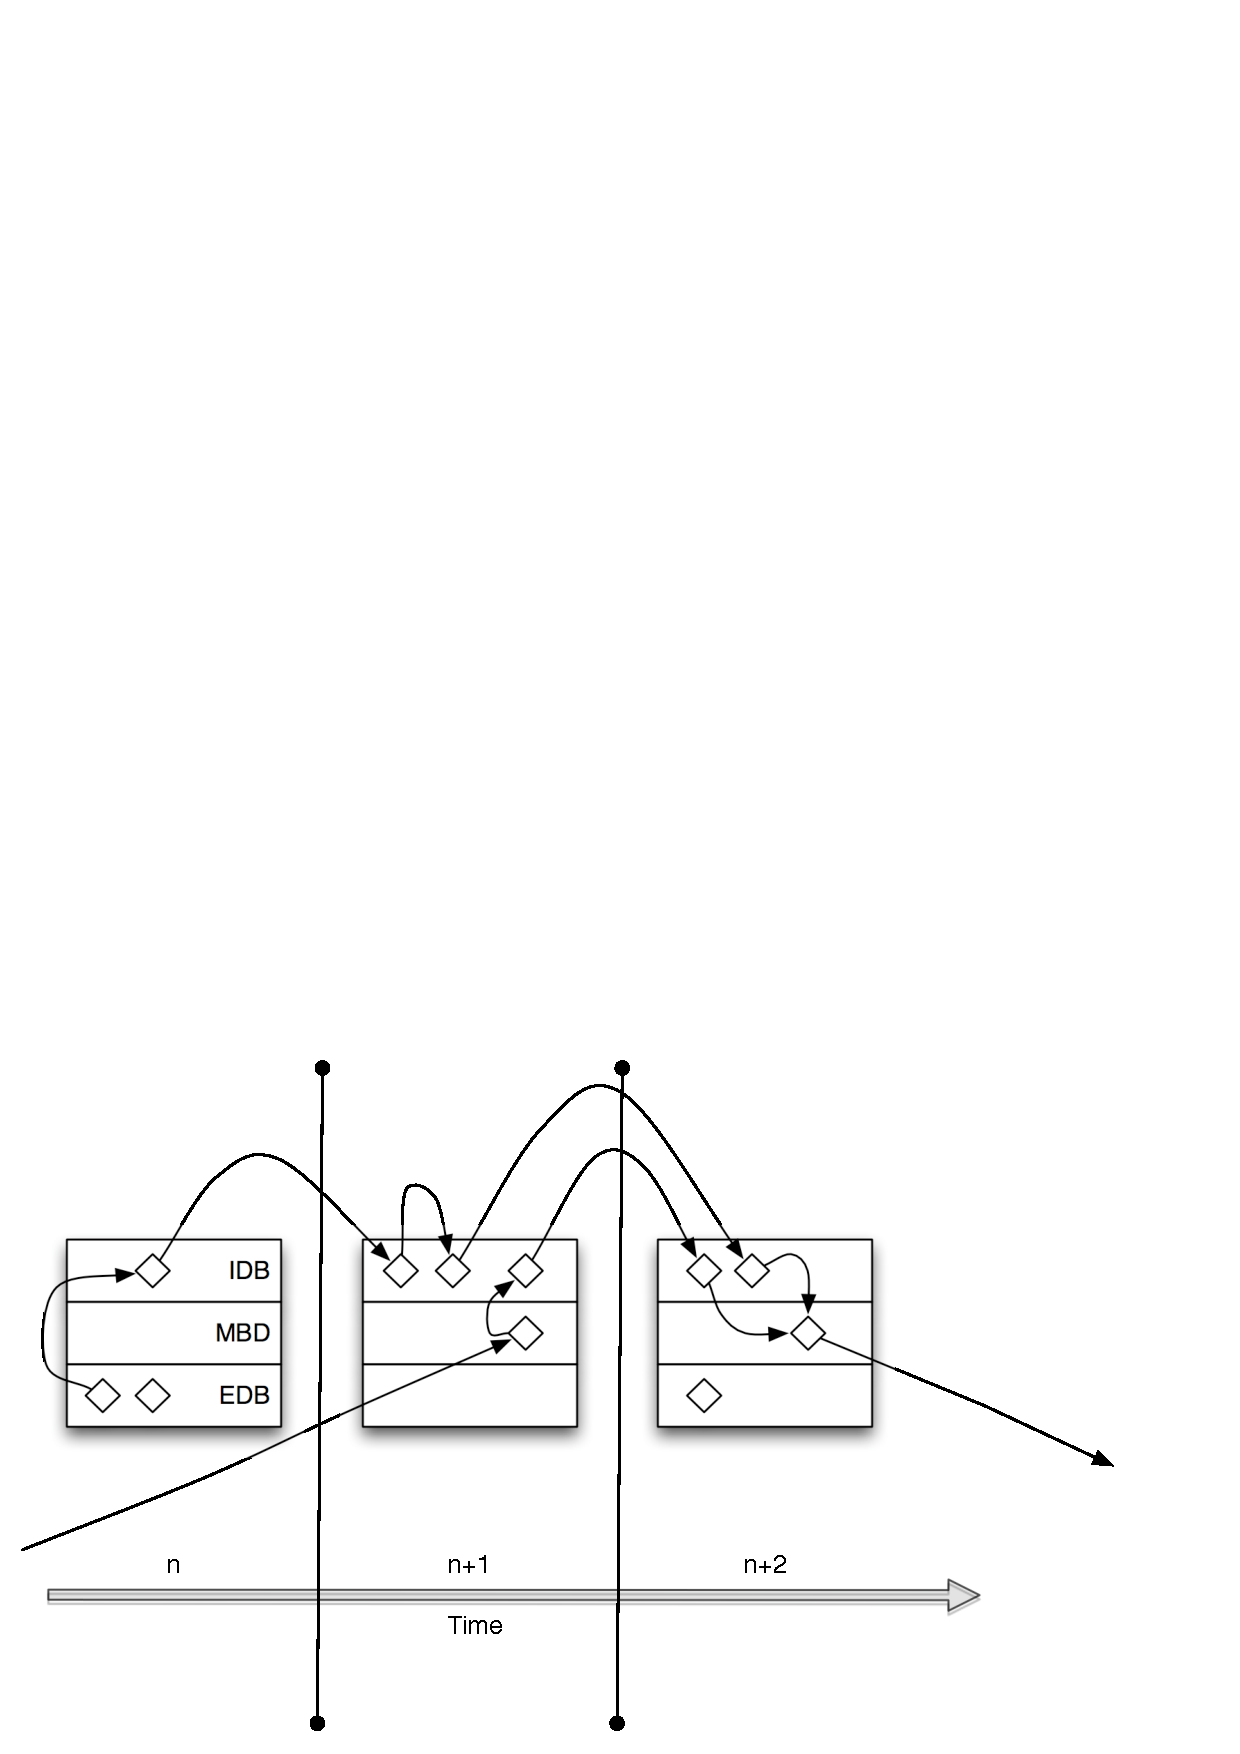
\includegraphics[width=1\linewidth]{edbidbmdb.pdf}
  \label{fig:edbidbmdb}
  \caption{Derivations across time in IDB and MDB relations.}
\vspace{-8pt}
\end{figure}


\section{Traces}

\paa{this section (its placement \emph{and} content) is somewhat problematic given the current structure
of the draft.  We've established the notion of finite prefixes of a (possibly infinite) EDB.  A trace is basically just
an interpretation (a set of ground atoms) -- by calling it a ``trace" we're connoting a post-hoc interpretation.
A trace that is just EDB is sufficient, given a program, to augment the trace with IDB and MDB atoms such that
the resulting trace is a model (by simply running a fixpoint computation).  For a program with no async rules, the EDB of input is sufficient to recreate the
program execution exactly -- that is to say, to reproduce the single minimal model of the program given the EDB.
It is \emph{not} sufficient to recreate the execution of a program with async rules: intuitively, we'd need to include in 
the trace the complete MDB, for every entry in it potentially corresponds to one of many possible minimal models.
perhaps we just want to show that there is a method (drop the async rules and run a fixpoint computation to generate
the IDB from MDB and EDB) to regenerate a "complete trace" (ie minimal model) from EDB $\cup$ MDB}

%Consider a non-empty EDB $E$, an empty MBD $M$ and IDB $I$ and a program $P$.  Evaluating $P$ against $E$ may derive facts in $M$ and $I$.

\begin{definition}
A \emph{trace} is any set of facts from the EDB, MDB or IDB of a Dedalus program evaluation.
\end{definition}

Any trace for a Dedalus instance $(P,E)$ is an interpretation of $(P,E)$.
%\wrm{lol, why do we need the notion of an incomplete trace?}

\begin{definition}
%
A \emph{complete trace} of an evaluation of a Dedalus instance is the union of
the given EDB with the derived IDB and MDB.
%
\end{definition}

\begin{lemma}
%
A complete trace of a Dedalus instance $(P,E)$ is its unique minimal model.
%
\end{lemma}

%\begin{lemma}
%%
%For any bound on $successor$, a complete trace of a Dedalus instance $(P,E)$ has a unique minimal model.
%%
%\end{lemma}

If we evaluate E given P, and P is stratifiable, the resulting set of ground atoms is a minimal model.
In our case, however, successor causes our EDB to be infinite, so the minimal model of any Dedalus program 
with temporal rules is potentially infinite.  \paa{but we'd like to show that a weaker property holds: that for any value $N$
in the \emph{successor} relation, the resulting program has a minimal model.}
\wrm{we either already showed this, or our theorems above are wrong.}


\begin{definition}
A \emph{minimal trace} is a subset of a complete trace that excludes any IDB ground atoms derived through an inductive
rule.
\end{definition}

A minimal trace of a Dedalus program $P$ is equivalent to the complete trace of which is is a subset -- the latter may be derived from the former by repeated
applications of inductive rules.  However, a given a Dedalus instance $(P, E)$ and a minimal trace T (where $E \subset T$), a fixpoint
computation will most likely \emph{not} yield a minimal model, because new tuples may be added to the MDB that represent a component 
of a different minimal model, and because these may affect the IDB.  The set of ground atoms $EDB \cup MDB_{old} \cup IDB_{new}$
\emph{may} may be a minimal model, iff $IDB_{new} = IDB_{old}$.  \paa{actually I am not sure if that is true}.  
$(EDB \cup MDB_{old} \cup IDB_{new} \cup IDB_{old})$ is certain to be a model, but is only minimal if $IDB_{new} \subset IDB_{old}$.

A minimal trace records the nondeterminism caused by the delay or reordering of async rules, and
is equivalent to the original program execution.  

\begin{definition}
A \emph{reduced trace} is a minimal trace with normalized time suffixes starting with 0 and increasing by 1 at each step.
\end{definition}

show a (trivial) procedure for reduction and make some claims about equivalences without entanglement.

\begin{definition}
A \emph{event trace} is a Dedalus EDB.
\end{definition}

An event trace and program P may be used to generate a new IDB and MDB.  The MDB is virtually certain to differ from that of another
execution, while the IDB may differ, depending on its dependency on the MDB.  The union of these three databases is of course a
minimal model, but probably not the same minimal model from another execution.  \paa{but can we say that it will often be true that if we project 
out the time attribute from every predicate, the minimal models will be the same? it won't always be true...}






\subsection{Queues}

%%Consider a trace of events to a 
Consider a predicate \emph{balance\_update} whose attributes are a string indicating the user, a floating point number
indicating the new balance and an integer indicating the order in which the updates were issued, according to some 
external clock or sequence.  

In this trace, all of the time suffixes are the same, e.g.

\begin{Dedalus}
balance\_update("bob", 100.00, 2355)@123;
balance\_update("bob", 75.00, 2358)@123;
balance\_update("alice", 0.00, 2377)@123;
balance\_update("bob", 10.00, 2455)@123;
\end{Dedalus}

Depending on the program that implements the balance update, several behaviors are possible.  We can see that in spite of their
coincidence in logical time, these events need to be processed in a data-dependent order, rather than as a set.  In-order tuple 
processing is difficult to express in Datalog generally, in part because the language has so notion of order of evaluation, except
the implicit ordering implied by stratification.

In the program below, we define a table \emph{m\_balance\_update} that we use as a queue to feed \emph{balance\_update}.  The queue must persist across
timesteps because it may take an unknown number of timesteps to drain it.  At each fixpoint, for each value of \textbf{A}, a single
tuple is projected into \emph{balance\_update} and atomically deleted from \emph{m\_balance\_update}, changing the value of the aggregate calculated at the
subsequent step:


\begin{Dedalus}

m\_balance\_update(A, B, C)@next \(\leftarrow\)
  m\_balance\_update(A, B, C),
  notin del\_m\_balance\_update(A, B, C);

omin(A, min<C>) \(\leftarrow\)
  m\_balance_update(A, _, C);

p(A, B, C)@next \(\leftarrow\)
  m\_balance\_update(A, B, C),
  omin(A, C);

del\_m\_balance\_update(A, B, C) \(\leftarrow\)
  m\_balance\_update(A, B, C),
  omin(A, C);
\end{Dedalus}

Under such a queueing discipline, deductive rules that are predicated on \emph{balance\_update} are constrained to consider only one tuple per fixpoint
per value of the variable \textbf{A}, thus implementing a per-user FIFO discipline.  To enforce a global FIFO ordering over \emph{balance\_update}, 
we may redefine \emph{omin} and any dependent rules to exclude the \textbf{A} atttribute.

A queue establishes a mapping between the local clock and the ordering domain of the input relation. By doing so, we are able to take
advantage of the natural ordering enforced by stratification over time, to enforce an ordering property over our input that is otherwise 
very difficult to express in a logic language.

\subsection{Lamport Clocks}

Implementing a Lamport Clock~\cite{timeclocks} is a special case of a queueing discipline as defined above.
Consider a predicate{m\_balance\_update} as defined above, but with an extra integer attribute that contains the logical transmission
time of the sender (via a message rule) of a given tuple.  For example, the sender's rule will look like: 

\paa{damn it!  we've sugared out N from the syntax!! now what?}

\begin{Dedalus}
entangle
m\_balance\_update(A, B, N)@async(N) \(\leftarrow\)
  send\_p(A, B);
\end{Dedalus}

Note that in the rule named \emph{entangle}, the time suffix is projected into the last attribute of \emph{m\_p}.  
This establishes an \emph{entanglement} between
the sender's local clock and the program dataflow.  The queueing discipline that implements a
Lamport clock is then:

\begin{Dedalus}

m\_balance\_update(A, B, C)@next \(\leftarrow\)
  m\_balance\_update(A, B, C),
  \(\lnot\) del\_m\_balance\_update(A, B, C);

omin(A, min<C>) \(\leftarrow\)
  m\_balance\_update(A, _, C);

lmax(max<C>) \(\leftarrow\)
  m\_balance\_update(_, _, C);

disentangle
balance_update(A, B)next \(\leftarrow\)
  m\_balance\_update(A, B, C)@N,
  omin(A, C)@N,
  lmax(L)@N,
  N > L;

del\_m\_balance\_update(A, B) :-
  m\_balance\_update(A, B),
  omax(B);
  
\end{Dedalus}

Note that the rule named \emph{disentangle} references the data elements $C$ and $L$, both of which
contain timestamps, and induces a \emph{balance\_update} tuple with timestamp $N+1$ only when $N > L$,
the highest of the timestamps in its message queue.  Under the distributed systems model of Lamport clocks, 
we expect the tuples in the message queue to  be from other hosts with independent clocks, sending messages 
over a medium that can delay or reorder them arbitrarily.  In order to make the necessary comparison between local
and remote clocks, it is necessary to reference the time suffix variable directly, rather than omitting it as we have done 
in all other Dedalus examples.

\subsection{Trace Entanglement}


\subsection{Reliable Broadcast}
Distributed systems cope with unreliable networks by using mechanisms like broadcast and consensus protocols, 
timeouts and retries, and often hide the nondeterminism behind these abstractions.  \lang supports these notions,
achieving encapsulation of nondeterminism while dealing explicitly with the uncertainty in the model.  Consider the simple
broadcast protocol below:

\begin{Dedalus}
sbcast(#Member, Sender, Message)@async \(\leftarrow\)
  smessage(#Agent, Sender, Message),
  members(#Agent, Member);

sdeliver(Member, Sender, Message) \(\leftarrow\)
  sbcast(Member, Sender, Message);
\end{Dedalus}

Assume the table \dedalus{members} is a persistent relation given to us, containing the broadcast 
membership list.  
%%The symbol \emph{\#} is used to indicate that the annotated attribute contains a network
%%address.  
The protocol is straightforward: if a tuple appears in \dedalus{smessage} (an EDB predicate), then
it will be sent to all members (a multicast).  The interpretation of the non-deterministic choice implied by the
\dedalus{@async} rule indicates that order and delivery (i.e. finite delay) are not guaranteed.

The program shown below makes use of the
multicast primitive provided by \dedalus{broadcast\_simple}, and uses it
to implement a basic reliable broadcast using a textbook
mechanism~\cite{mullender} that assumes any node that fails to receive
a message sent to it has failed.  When broadcast completes, all nodes
that have not failed have received the message.

Our simple two-rule broadcast program is augmented with the following rules, so that if a node receives a message, it 
also multicasts it to every member \emph{before} delivering the message locally:

\begin{Dedalus}
smessage(Agent, Sender, Message)  \(\leftarrow\)
  rmessage(Agent, Sender, Message);

buf_bcast(Sender, Me, Message)  \(\leftarrow\)
  sdeliver(Me, Sender, Message);

smessage(Me, Sender, Message)  \(\leftarrow\)
  buf_bcast(Sender, Me, Message);

rdeliver(Me, Sender, Message)@next  \(\leftarrow\)
  buf_bcast(Sender, Me, Message);
\end{Dedalus}

Note that all network communication is initiated by the
\dedalus{@async} rule from the original simple broadcast.  The \dedalus{@next} is
required in the \dedalus{rdeliver} definition in order to prevent nodes from
taking actions based upon the broadcast before it is guaranteed to
meet the reliability guarantee.

Implementing other disciplines like FIFO and atomic broadcast and
consensus are similar exercises, requiring the use of ordered queueing
and sequences.

\section{Related Work}

\subsection{Concurrency control}
The importance of commutative operations has long been recognized by work in the
distributed systems, data management, and groupware communities.

\subsection{Non-monotonicity in deductive databases}
Adding non-monotonic operators (e.g., aggregation and negation) to Datalog
increases the expressiveness of the language but introduces significant
complexities: care must be taken to ensure that the resulting language has a
semantics that is well-defined, intuitive to the user, and amenable to efficient
evaluation. A straightforward approach is to disallow recursion through
aggregation or negation, which admits only the class of so-called ``stratified
programs''~\cite{Apt1988}. Many attempts have been made to assign a semantics to
larger classes of programs (e.g.,~\cite{Gelfond1988,Ross1990,VanGelder1991}).

The observation that many uses of aggregation and negation have a ``monotonic''
flavor has been made before.

% CRDTs
% Work on semantics-aware concurrency control
% Operational transformations
% Ross & Sagiv on lattices
% Kostler et al. on differential fixpoint + subsumption

\section{Future Work}
\label{future}
The current implementation and design of our system shows that declarative systems can be used to implement algorithms that perform distributed spam filtering. The results of the distributed implementation of \emph{SpamTracker}~\cite{bb} using P2 show signs of detecting spam and can be used with existing techniques to improve spam filtering. In this section, we discuss some areas of improvement to the system design and algorithm, and how the system can be made deployable, scalable and used in real-time. We also discuss some security and privacy concerns relating to spammers evading these clustering techniques and domains sharing information securely.\\ 
\emph{Scalability and Temporal Compression:} The clustering algorithm requires aggregation of sending pattern of all IP addresses across multiple domains in \emph{$\bigtriangleup t$} time interval. This aggregation results in a \emph{n}x\emph{d} matrix where \emph{n} is extremely large. Due to this, the application is not scalable and may use high amount of bandwidth for aggregating information. We plan to use \emph{temporal compression} \cite{baysail} heuristics to reduce the amount of information that has to be sent after each \emph{$\bigtriangleup t$} time interval. Temporal compression involves sharing information only if the data has changed beyond some threshold since the last update interval. In our setting, information about a new spammer's activity at a domain is only sent if the current clusters' sending patterns are different from before over a threshold.\\
\emph{Deployability:} In the current design of the system we use a set of separate super-nodes to perform clustering. For deployment and use of the system in the real-world we need to understand how well does the system performs in terms of the number of super-nodes. Is it better to have large number of super-nodes with less information per node or have small number of super-nodes but more information per node? What is the trade-off in selecting either of the designs? We also need to analyze different settings where the super-nodes are either domain mail server or nodes in an enterprise with which domain mail servers share information.\\
\emph{Optimizing bandwidth:} The number of messages sent across  the network depends on the number of non-zero similarities among the IP addresses. If there is a large number of such similarities, bandwidth issues may arise. We need to perform optimizations that reduce the message cost. One method, that reduces the number of messages transferred, sends only messages to IP addresses that have a similarity, a responsibility and a availability above a certain threshold. We plan to evaluate how well the algorithm will work with these optimizations. Such optimization are very easy to implement in P2.\\
\emph{Privacy and Evasion:} Adversaries may corrupt the information sent by domains, that contain sending patterns of spammers. To improve the robustness of the system, information can be shared only by trusted domain mail servers, and the communication can take place using a secure channel. The clustering algorithm collects information every \emph{$\bigtriangleup t$} hours. Attackers can evade detection by spreading their activity over a large \emph{$\bigtriangleup t$} time interval. This raises the need to dynamically alter \emph{$\bigtriangleup t$} time interval periodically.

\section*{Acknowledgments}
We would like to thank Peter Bailis, Ali Ghodsi, David Maier, and Matei Zaharia
for their helpful feedback on this paper.  This work was supported by the
Natural Sciences and Engineering Research Council of Canada.

\bibliographystyle{abbrv}
\bibliography{datalog2.0,declarativity}



\end{document}
